\documentclass{standalone}
\usepackage[dvipsnames,svgnames,x11names]{xcolor}
\usepackage{tikz}
\usepackage{pgfplots}
\pgfplotsset{compat = 1.12}
\usepackage{../thesismath}
\begin{document}
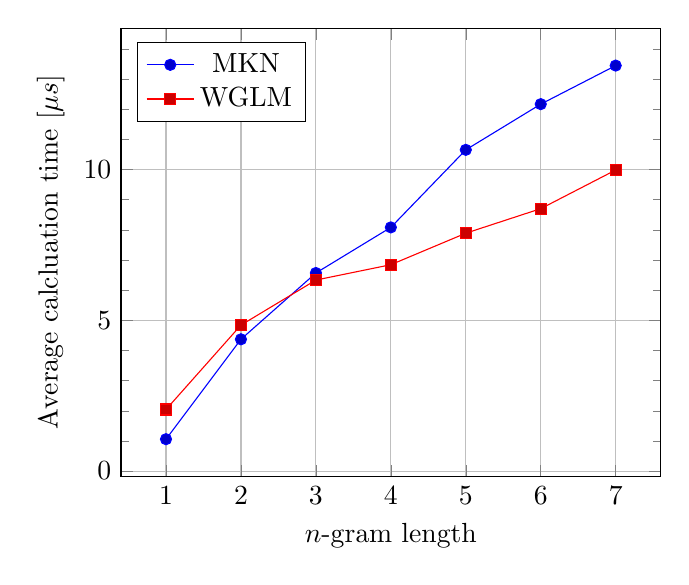
\begin{tikzpicture}[baseline]

\begin{axis}[
  xlabel = {$n$-gram length},
  ylabel = {Average calcluation time [${\mu}s$]},
  minor y tick num = 4,
  grid = major,
  legend entries = {{MKN}, {WGLM}},
  legend pos = north west,
]

% MLE
%\addplot table {
%  n us
%  1 3.622
%  2 3.776
%  3 4.084
%  4 5.637
%  5 7.409
%  6 10.897
%  7 12.816
%};

% MKN
\addplot table {
  n us
  1 1.058
  2 4.371
  3 6.570
  4 8.083
  5 10.655
  6 12.171
  7 13.450
};

% WMKN
\addplot table {
  n us
  1 2.042
  2 4.842
  3 6.336
  4 6.845
  5 7.890
  6 8.704
  7 9.986
};

\end{axis}

\end{tikzpicture}
\end{document}
